\documentclass[]{article}
\usepackage[T1]{fontenc}
\usepackage{lmodern}
\usepackage{amssymb,amsmath}
\usepackage{ifxetex,ifluatex}
\usepackage{fixltx2e} % provides \textsubscript
% use microtype if available
\IfFileExists{microtype.sty}{\usepackage{microtype}}{}
\ifnum 0\ifxetex 1\fi\ifluatex 1\fi=0 % if pdftex
  \usepackage[utf8]{inputenc}
\else % if luatex or xelatex
  \usepackage{fontspec}
  \ifxetex
    \usepackage{xltxtra,xunicode}
  \fi
  \defaultfontfeatures{Mapping=tex-text,Scale=MatchLowercase}
  \newcommand{\euro}{€}
\fi
\usepackage{listings}
\usepackage{graphicx}
% We will generate all images so they have a width \maxwidth. This means
% that they will get their normal width if they fit onto the page, but
% are scaled down if they would overflow the margins.
\makeatletter
\def\maxwidth{\ifdim\Gin@nat@width>\linewidth\linewidth
\else\Gin@nat@width\fi}
\makeatother
\let\Oldincludegraphics\includegraphics
\renewcommand{\includegraphics}[1]{\Oldincludegraphics[width=\maxwidth]{#1}}
\ifxetex
  \usepackage[setpagesize=false, % page size defined by xetex
              unicode=false, % unicode breaks when used with xetex
              xetex]{hyperref}
\else
  \usepackage[unicode=true]{hyperref}
\fi
\hypersetup{breaklinks=true,
            bookmarks=true,
            pdfauthor={Jörg Kuharev},
            pdftitle={ISOQuant usage guide},
            colorlinks=true,
            urlcolor=blue,
            linkcolor=magenta,
            pdfborder={0 0 0}}
\setlength{\parindent}{0pt}
\setlength{\parskip}{6pt plus 2pt minus 1pt}
\setlength{\emergencystretch}{3em}  % prevent overfull lines
\usepackage[left=2cm,right=1.5cm,top=1.5cm,bottom=1.5cm]{geometry}
% \setlength{\parindent}{0.25in}
\setlength{\parskip}{0.4cm}
\pagestyle{plain}

%\renewcommand{\figurename}{Abb.}
%\renewcommand{\tablename}{Tab.}
%\renewcommand{\listfigurename}{Abbildungsverzeichnis}
%\renewcommand{\listtablename}{Tabellenverzeichnis}
%\renewcommand{\refname}{Literaturverzeichnis}
\renewcommand{\contentsname}{Table of contents}

\renewcommand{\baselinestretch}{1.0}\normalsize

\title{ISOQuant usage guide}
\author{Jörg Kuharev}
\date{\today}

\begin{document}
\maketitle

{
\hypersetup{linkcolor=black}
\tableofcontents
}
\begin{center}\rule{3in}{0.4pt}\end{center}

\clearpage

\section{About usage guide}

This document describes how to operate ISOQuant.

\section{Installation}

For installing ISOQuant application, please read
\lstinline!ISOQuant installation guide! and follow instructions.

\section{Purpose of ISOQuant}

The basic idea behind ISOQuant is to reduce data analysis time and also
to ensure constant analysis quality by automating standard analysis
steps applied to LC-MS based label-free proteomics data.

\section{Workflow}

\subsection{Overview}

ISOQuant extracts preprocessed data from vendor software (Waters PLGS),
and transfers extracted information into a relational MySQL database.
Once data is transferred, ISOQuant applies a set of statistical analysis
steps to it and reports analysis results in human readable, common file
formats.

\subsection{Steps}

Main workflow contains following steps:

\begin{itemize}
\item
  PLGS root folder selection
\item
  MySQL database connection
\item
  Parameter configuration
\item
  Project selection
\item
  Processing type selection
\item
  Project design or Expression Analysis selection
\item
  Automated processing
\item
  Report creation
\end{itemize}

\section{Workflow steps explained}

\subsection{PLGS root folder selection}

On the main view of ISOQuant, click on `select PLGS root folder' button
(figure \ref{pic:GUI}, item 3) to initiate root folder selection. From
the appearing folder selection dialog, choose the correct path to PLGS
root folder, e.g.~C:\textbackslash{}PLGS2.4\textbackslash{}root. Do not
select the PLGS folder, nor one of the project folders inside the root.
When you have selected a valid root folder, ISOQuant explores contained
projects and shows them as a list inside the
\lstinline!projects in PLGS root folder! container.

\begin{figure}[htbp]
\centering
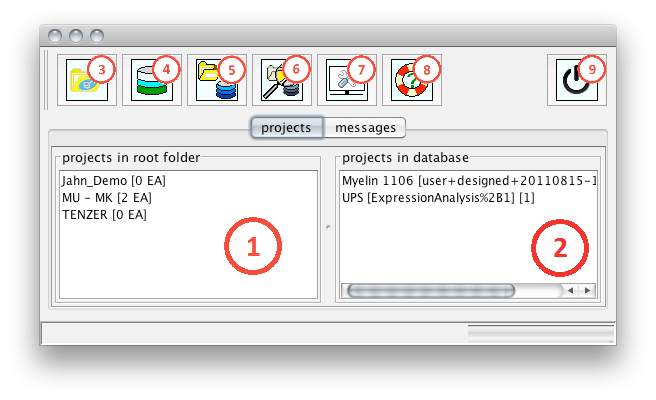
\includegraphics{assets/isoquant/pics/gui.png}
\caption{the main view of ISOQuant \label{pic:GUI}}
\end{figure}

\subsection{MySQL database connection}

On the main view of ISOQuant, click `connect database' button (figure
\ref{pic:GUI}, item 4) and type requested accession data into
appropriate fields on appearing dialog (figure \ref{pic:dbDialog}). Once
ISOQuant has successfully connected to a MySQL database, it shows a list
of previously imported projects inside the
\lstinline!projects in MySQL database! (figure \ref{pic:GUI}, item 2)
container.

\begin{figure}[htbp]
\centering
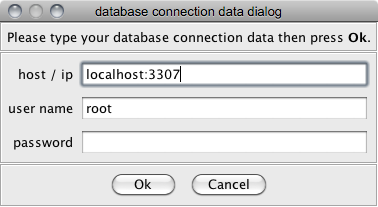
\includegraphics{assets/isoquant/pics/db_dialog.png}
\caption{database connection dialog \label{pic:dbDialog}}
\end{figure}

\subsection{Parameter configuration}

The behavior and the appearance of ISOQuant as well as the attributes of
its processing steps may be adapted by editing ISOQuant's configuration
file \lstinline!isoquant.ini!. The easiest way to edit the configuration
file is to use the built-in configuration editor (figure
\ref{pic:cfgEditor}). Which is accessible from ISOQuant's GUI by
clicking \lstinline!edit configuration! button (figure \ref{pic:GUI},
item 7) . Please see \lstinline!ISOQuant configuration guide! for
detailed explanation of attributes and possible values.

\begin{figure}[htbp]
\centering
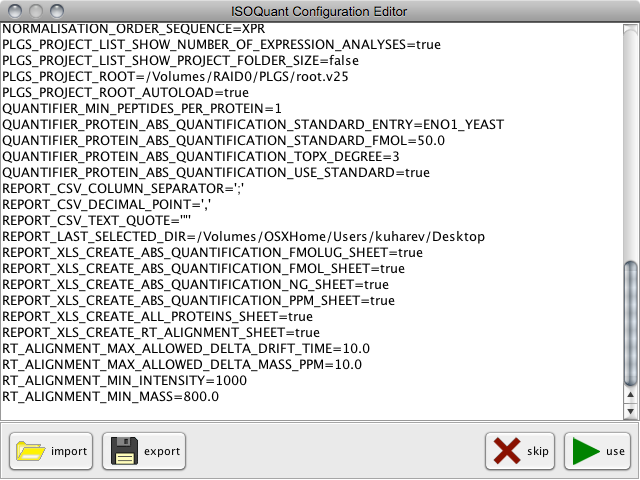
\includegraphics{assets/isoquant/pics/configuration_editor.png}
\caption{built-in configuration editor \label{pic:cfgEditor}}
\end{figure}

\subsection{Project selection}

Projects to be processed with ISOQuant may be selected from
\lstinline!projects in PLGS root folder! container (figure
\ref{pic:GUI}, item 1) by left clicking them. Multiple projects could be
selected by holding \lstinline!Shift! or \lstinline!Control! and left
clicking them.

\subsection{Processing type selection}

Right click on selected projects and choose
\lstinline!import and process! from appearing context menu (figure
\ref{pic:fsMenu}). The appearing submenu offers a set of predefined
processing pipelines for processing data in different ways depending on
user choice and preprocessing status.

\begin{figure}[htbp]
\centering
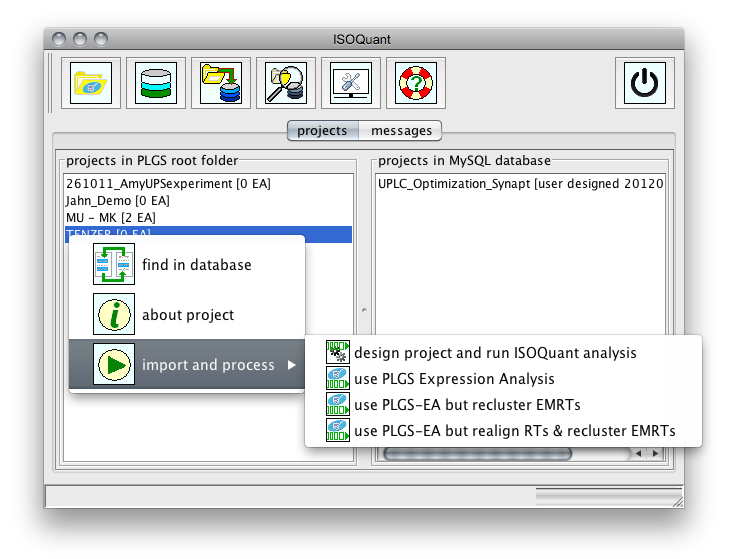
\includegraphics{assets/isoquant/pics/fs_context.png}
\caption{context menu for \lstinline!projects in PLGS root folder!
\label{pic:fsMenu}}
\end{figure}

\subsection{Project design or Expression Analysis selection}

\subsubsection{Project design}

Project designer dialog (figure \ref{pic:prjDesigner}) shows for each
selected project the original PLGS project structure and the targeted
ISOQuant project structure, which is redefineable by drag-and-drop.

\begin{figure}[htbp]
\centering
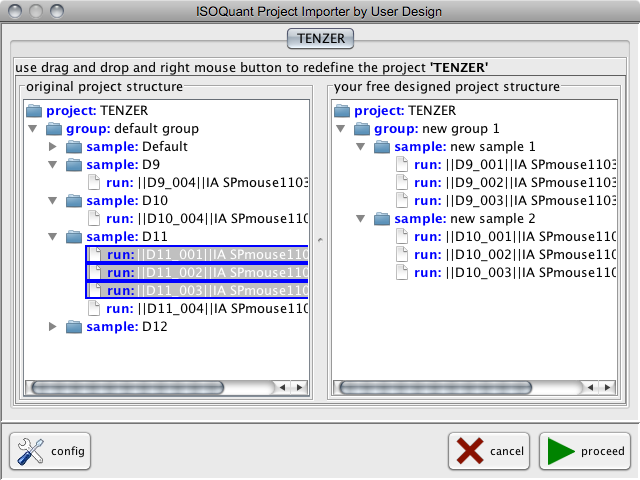
\includegraphics{assets/isoquant/pics/project_designer.png}
\caption{project designer \label{pic:prjDesigner}}
\end{figure}

\subsubsection{Expression Analysis selection}

For each selected project every contained Expression Analysis may be
selected to be imported and processed by ISOQuant by using
\lstinline!Expression Analysis Selector! (figure \ref{pic:eaSelector}).

\begin{figure}[htbp]
\centering
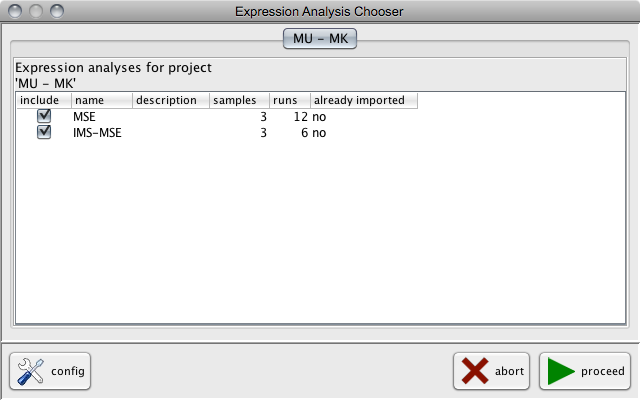
\includegraphics{assets/isoquant/pics/expression_analysis_selector.png}
\caption{Expression Analysis Selector \label{pic:eaSelector}}
\end{figure}

\subsection{Automated processing}

Automated processing of user chosen contents is initiated after project
design or Expression Analysis selection is done. Depending on user
choice, data is processed by different predefined analysis pipelines.

\subsection{Report creation}

After successfully importing and processing data, newly processed
projects appear inside \lstinline!projects in MySQL database! container
(figure \ref{pic:GUI}, item 2). By selecting and right clicking on one
of them, its processing results may be reported to a file (figure
\ref{pic:dbMenu}). Different types of report are available offering
different points of view at the analysis results.

\begin{figure}[htbp]
\centering
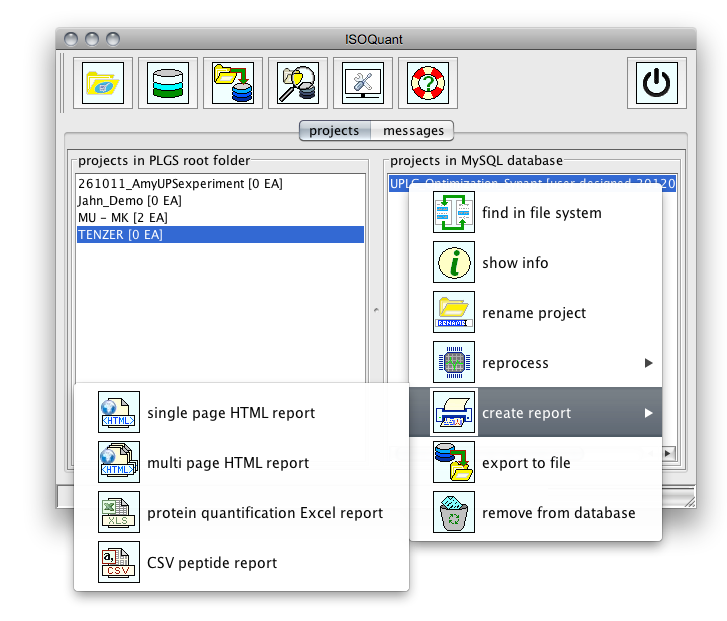
\includegraphics{assets/isoquant/pics/db_context.png}
\caption{context menu for \lstinline!projects in ISOQuant database!
\label{pic:dbMenu}}
\end{figure}

\end{document}
